\documentclass[14pt,utf8,notheorems,compress,t]{beamer}
\usepackage{etex}

\usepackage[english]{babel}

\RequirePackage[all]{xy}
\usepackage{mathtools}
\usepackage{booktabs}
\usepackage{array}
\usepackage{ragged2e}
\usepackage{multicol}
\usepackage{tabto}
\usepackage{xstring}

\usepackage[protrusion=true,expansion=false]{microtype}

\setlength\parskip{\medskipamount}
\setlength\parindent{0pt}

\renewcommand{\U}{\mathcal{U}}
\newcommand{\NN}{\mathbb{N}}
\newcommand{\id}{\mathrm{id}}
\newcommand{\ZZ}{\mathbb{Z}}
\newcommand{\RR}{\mathbb{R}}
\newcommand{\Id}{\mathrm{Id}}
\newcommand{\fst}{\mathsf{fst}}
\newcommand{\snd}{\mathsf{snd}}
\newcommand{\inv}{\mathsf{inv}}
\newcommand{\refl}{\mathsf{refl}}
\newcommand{\ap}{\mathsf{ap}}
\renewcommand{\succ}{\mathsf{succ}}
\newcommand{\seg}{\mathsf{seg}}
\newcommand{\base}{\mathsf{base}}
\newcommand{\lloop}{\mathsf{loop}}
\newcommand{\ua}{\mathsf{ua}}
\newcommand{\code}{\mathsf{code}}
\newcommand{\surf}{\mathsf{surf}}
\newcommand{\merid}{\mathsf{merid}}
\newcommand{\N}{\mathsf{N}}
\renewcommand{\S}{\mathsf{S}}
\newcommand{\Cyl}{\mathrm{Cyl}}
\newcommand{\IsContr}{\mathsf{IsContr}}
\newcommand{\IsMereProp}{\mathsf{IsMereProp}}
\newcommand{\IsSet}{\mathsf{IsSet}}
\newcommand{\IsEquiv}{\mathsf{IsEquiv}}
\newcommand{\LEM}{\mathsf{LEM}}
\newcommand{\UIP}{\mathsf{UIP}}
\newcommand{\fib}{\mathsf{fib}}
\newcommand{\List}{\mathsf{List}}
\newcommand{\defeq}{\vcentcolon=}
\newcommand{\defeqv}{\vcentcolon\equiv}
\newcommand{\ct}{%
  \mathchoice{\mathbin{\raisebox{0.5ex}{$\displaystyle\centerdot$}}}%
             {\mathbin{\raisebox{0.5ex}{$\centerdot$}}}%
             {\mathbin{\raisebox{0.25ex}{$\scriptstyle\,\centerdot\,$}}}%
             {\mathbin{\raisebox{0.1ex}{$\scriptscriptstyle\,\centerdot\,$}}}
}
\renewcommand{\_}{\mathpunct{.}}

\newtheorem{axiom}{Axiom}

\title{Double-negation translation and\\ CPS transformation}
\author[Ingo Blechschmidt]{\vspace{-1em}\\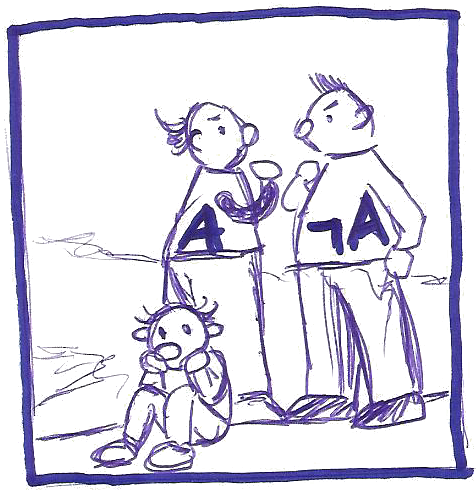
\includegraphics[scale=0.6]{lem} \\[0.5em] Ingo Blechschmidt \\[-0.3em] {\scriptsize June 3rd, 2015}}
\date{June 3d, 2015}

\usetheme{Warsaw}
\usecolortheme{seahorse}
%\usefonttheme{default}?
\usepackage[T1]{fontenc}
\usepackage{libertine}
\usefonttheme{serif}
%\usepackage{libertine}?
%\usepackage{mathpazo}
\useinnertheme{rectangles}

\setbeamertemplate{title page}[default][colsep=-1bp,rounded=false,shadow=false,bg=white]
\setbeamertemplate{frametitle}[default][bg=red,colsep=-2bp,rounded=false,shadow=false,center]
\setbeamertemplate{blocks}[rounded][shadow=false]

\setbeamertemplate{frametitle}{%
  \vskip1em%
  \leavevmode%
  \begin{beamercolorbox}[dp=1ex,center]{}%
      \usebeamercolor[fg]{item}{\textbf{\textsf{\Large \insertframetitle}}}
  \end{beamercolorbox}%
}

\setbeamertemplate{footline}{%
  \leavevmode%
  \hfill%
  \begin{beamercolorbox}[ht=2.25ex,dp=1ex,right]{}%
    \usebeamerfont{date in head/foot}
    \insertframenumber\,/\,\inserttotalframenumber\hspace*{1ex}
  \end{beamercolorbox}%
  \vskip0pt%
}

\setbeamertemplate{headline}{}
\setbeamertemplate{navigation symbols}{}

\newcommand{\floatbox}[3]{%
  \raisebox{0pt}[0pt][0pt]{%
    \begin{picture}(0,0)(#1,#2)#3\end{picture}\leavevmode%
  }%
}

\newcommand{\backupstart}{
  \newcounter{framenumberpreappendix}
  \setcounter{framenumberpreappendix}{\value{framenumber}}
}
\newcommand{\backupend}{
  \addtocounter{framenumberpreappendix}{-\value{framenumber}}
  \addtocounter{framenumber}{\value{framenumberpreappendix}} 
}

\newcommand{\hil}[1]{{\usebeamercolor[fg]{item}{\textbf{#1}}}}

\newcommand{\img}[3]{\begin{center}\includegraphics[scale=#1]{#2}\\\scriptsize#3\end{center}}
%\newcommand{\imageslide}[3]{\frame{\frametitle{#1}\img{#2}{#3}}}

\IfSubStr{\jobname}{\detokenize{nonotes}}{
  \setbeameroption{hide notes}
}{
  \setbeameroption{show notes}
}
\setbeamertemplate{note page}[plain]

\newenvironment{changemargin}[2]{%
  \begin{list}{}{%
    \setlength{\topsep}{0pt}%
    \setlength{\leftmargin}{#1}%
    \setlength{\rightmargin}{#2}%
    \setlength{\listparindent}{\parindent}%
    \setlength{\itemindent}{\parindent}%
    \setlength{\parsep}{\parskip}%
  }%
  \item[]}{\end{list}}

\graphicspath{{images/}}

\begin{document}

\frame[plain,c]{
  \begin{center}
    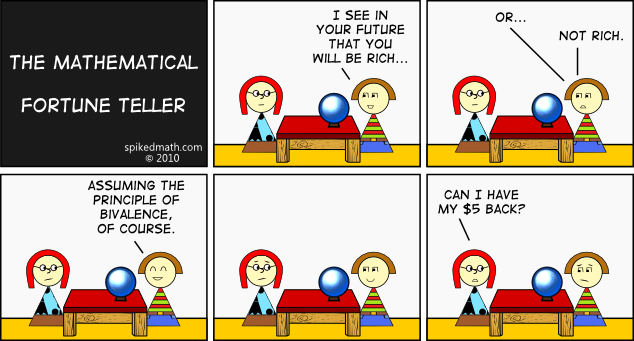
\includegraphics[scale=0.65]{fortune-teller}
  \end{center}
}

\frame{\titlepage}

\note{\fontsize{8pt}{9.6}\selectfont
  \begin{center}\large\textbf{Abstract}\end{center}

  \begin{changemargin}{2.5em}{2.5em}
    \justifying
    Constructive mathematicians don't use the law of excluded middle, which
    approximately says that for any proposition~$P$, either~$P$ is true or~$\neg P$
    is true. Several advantages emerge from this rejection, for instance one
    can mechanically extract algorithms from constructive proofs of existence
    statements and rigorously work with non-standard \emph{dream axioms} which are
    plainly false in classical mathematics, such as \emph{any function is
    smooth}.

    For communicating with classicial mathematicians, constructive
    mathematicians can employ the \emph{double-negation translation}. This
    device associates to any formula a translated formula in such a way that
    a given formula holds classically if and only if its translation holds
    constructively.

    The talk will give an introduction to these topics and discuss the
    intriguing relationship of the double-negation translation with the
    well-known con\-tin\-u\-a\-tion-pas\-sing style transformation: In some sense, they are
    the same. This is a beautiful facet of \emph{computational trinitarianism}.

    For the first part of the talk, no background in formal logic or
    constructive mathematics is required. For the second part of the talk,
    one should be vaguely familiar with the continuation-passing style
    transformation.
  \end{changemargin}
}

\frame{\frametitle{Outline}\begin{itemize}\item[]\tableofcontents\end{itemize}}

\section{Constructive mathematics}

\subsection{The law of excluded middle}

\newcommand{\constructiveinterpretation}{
  \begin{minipage}{0.99\textwidth}
    \begin{block}{\centering Constructive interpretation}
      \begin{description}\small
        \item[$\bot$] There is a contradiction.
        \item[$A \wedge B$] We have evidence for $A$ and for $B$.
        \item[$A \vee B$] We have evidence for $A$ or for $B$.
        \item[$A \Rightarrow B$] We can transform evidence for $A$ into
        one for $B$.
        \item[$\forall x{:}X\_ A(x)$] Given $x:X$, we can construct evidence
        for $A(x)$.
        \item[$\exists x{:}X\_ A(x)$] We have an $x:X$ together with evidence
        for $A(x)$.
      \end{description}
    \end{block}
  \end{minipage}
}

\frame{\frametitle{The law of excluded middle}
  \centering
  ``For any formula~$A$, we may deduce~$A \,\vee\, \neg A$.''

  \medskip
  Classical mathematics $=$ \\
  intuitionistic logic $+$ law of excluded middle.

  \vfill

  \only<1>{
    \begin{minipage}{0.8\textwidth}
      \begin{block}{\centering Classical interpretation}
        \begin{description}\small
          \item[$\bot$] There is a contradiction.
          \item[$A \wedge B$] $A$ and $B$ are true.
          \item[$A \vee B$] $A$ is true or $B$ is true.
          \item[$A \Rightarrow B$] If~$A$ holds, then also~$B$.
          \item[$\forall x{:}X\_ A(x)$] For all~$x:X$ it holds that~$A(x)$.
          \item[$\exists x{:}X\_ A(x)$] There is an $x:X$ such that~$A(x)$.
        \end{description}
      \end{block}
    \end{minipage}
  }
  \only<2>{
    \constructiveinterpretation
  }
  \par
}

\note{\justifying
  More precisely, one should say: Classical mathematics $=$ intuitionistic
  logic $+$ law of excluded middle $+$ a set theory including the axiom of
  choice.

  The constructive interpretation of the axiom of excluded middle is: For any
  formula~$A$, we have evidence for~$A$ or for~$\neg A$. This is an absurd
  statement.

  Several years ago a video showing Kate Moss consuming drugs surfaced.
  From the video it was clear that the drugs were either of some type~$A$ or of some type~$B$,
  but there was no direct evidence for either type.
  Kate Moss was not prosecuted; in this sense, Great Britain's judicial system
  operated intuitionistically.
  \par
}

\subsection{Interpretation of intuitionistic logic}

\frame{\frametitle{Doubly-negated statements}
  \centering
  ``$\neg\neg A$'' means: There is no evidence for~$\neg A$.

  Trivially, we have $A \Longrightarrow \neg\neg A$. \\
  We can't deduce $\neg\neg A \Longrightarrow A$.

  \vfill
  \constructiveinterpretation
  \par
}

\note{\justifying
  If we know that the key to our apartment has to be somewhere in the
  apartment (since we used it to enter last night) but we can't find it, we can
  constructively only justify
  \[ \neg\neg \exists x\_ \text{the key is at position $x$}, \]
  not the stronger statement
  \[ \phantom{\neg\neg} \exists x\_ \text{the key is at position $x$}. \]
}

\subsection{Applications}

\frame{\frametitle{Applications}
  \begin{changemargin}{-0.5em}{-0.5em}
    \only<1>{
      Intuitionistic logic \ldots
      \begin{itemize}
        \item can guide you to more elegant proofs, \\[0.2em]
        \item is good for the mental hygiene, and \\[0.2em]
        \item allows to make finer distictions.
      \end{itemize}
    }
    \only<2>{
      \begin{itemize}
        \item We can \hil{mechanically extract algorithms} from intuitionistic proofs
        of existence statements. \\[0.2em]
        \item The \hil{internal language of toposes} is intuitionistic.
        \\[0.2em]
        \item \hil{Dream mathematics} works only intuitionistically.
      \end{itemize}
    }
  \end{changemargin}

  \vfill
  \centering
  \only<1>{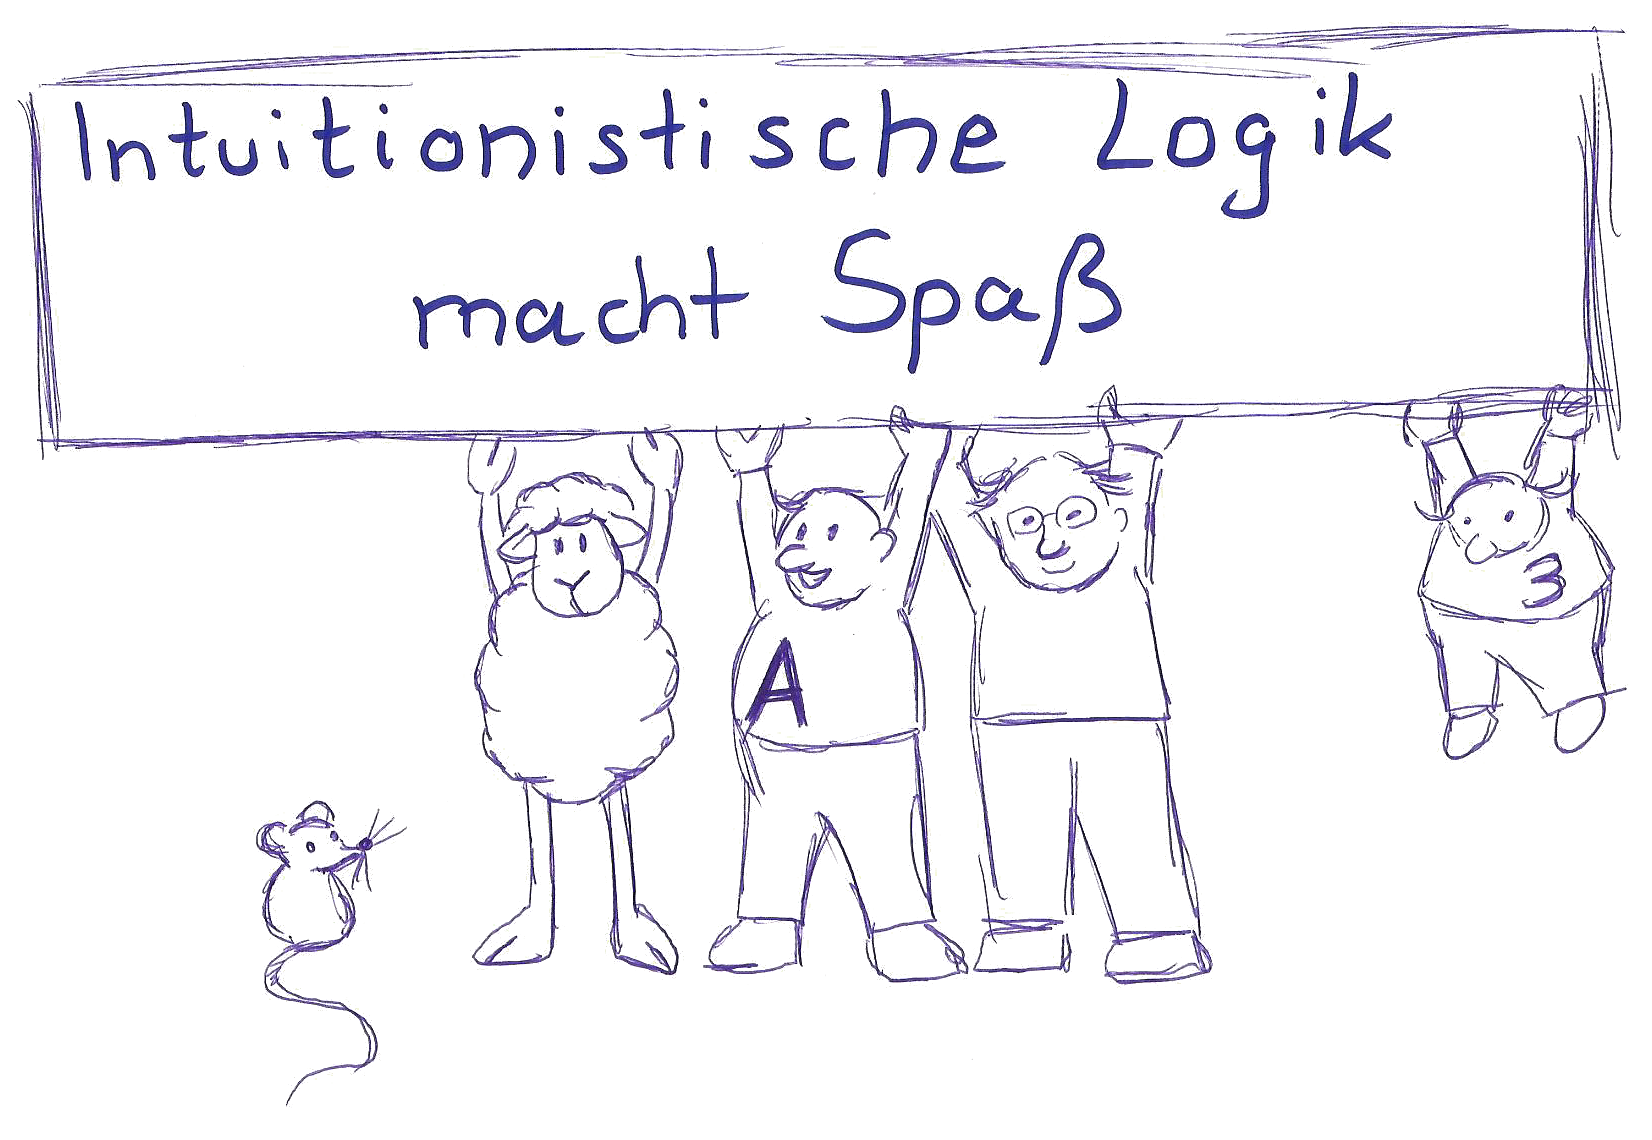
\includegraphics[height=5cm]{fun}}
  \only<2>{%
    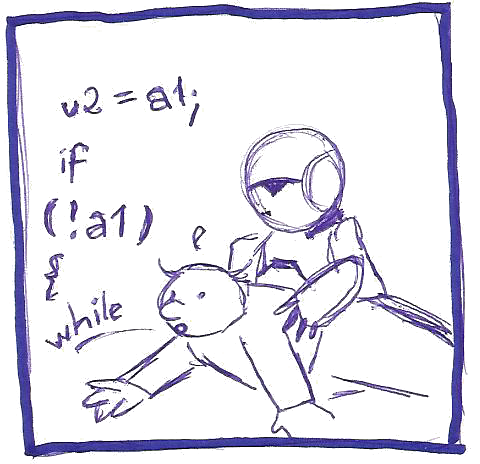
\includegraphics[height=3cm]{program-extraction}
    \hfill
    
\includegraphics[height=3cm]{constructive-maths}
    \hfill
    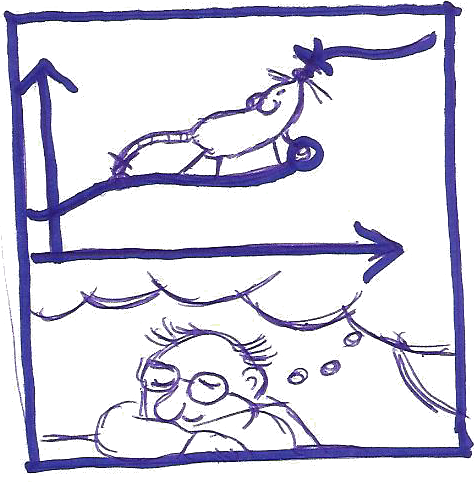
\includegraphics[height=3cm]{dream-maths}
  }
  \par
}

\section{The double-negation translation}

\subsection{The double-negated law of excluded middle}

\subsection{The fundamental result}

\section{Continuations}

\end{document}

Start with the Spiked Math comic, of course.

1. Constructive mathematics
   * LEM
   * (Informal) BKH interpretation
   * Applications

2. The double-negation translation
   * Proof of neg neg (phi v neg phi)
   * Game-theoretical intepretation
   * The translation and the fundamental result

3. Relation to continuations
   * ...

4. Outlook
   * CPS transformation = Yoneda embedding
   * Box-translation for arbitrary modal operators Box
   * negneg-sheafification?
